\chapter{Preliminary results} \label{ch-results}

\section{Variance deconvolution for uncertainty quantification}\label{sec:results-uq}
\subsection{Problem description}
To verify the variance deconvolution method, we applied the UQ variance estimator in Eq.~\eqref{eq:var-deconv} (repeated below for convenience) to a radiation transport problem with an analytic solution to compare against. We solve the one-dimensional, neutral-particle, mono-energetic, steady-state radiation transport equation with a normally incident beam source of magnitude one:
\begin{gather}
	\label{eq:transport}
 	\mu \frac{\partial \psi(x,\mu)}{\partial x} + \Sigma_t(x) \, \psi(x,\mu) =  \int_{-1}^{1} d\mu' \psi(x,\mu') \frac{\Sigma_s(x,\mu' \rightarrow \mu)}{2} , \\
	0 \leq x \leq L; \quad -1 \leq \mu \leq 1, 
\end{gather}
\noindent where $\psi(x, \mu)$ is angular flux, $\Sigma_t(x)$ is total cross section, $\Sigma_s(x,\mu)$ is scattering cross section, and $x$ and $\mu$ respectively denote dependence on space and angle. The problem is a slab geometry with fixed boundaries $x \in [0,L]$ and fixed boundaries between material regions. The problem is solved for two different scenarios: attenuation-only in which $\Sigma_s(x,\mu) = 0$, and with both attenuation and isotropic scattering. 
We introduce stochasticity into the problem via the total cross section and, for the problem with scattering, the scattering ratio. As with the derivations in Section~\ref{sec:method-uq}, we represent the stochasticity with the variable $\xi$. For both scenarios, the total cross section of each material is assumed to be uniformly distributed. In the scenario which also involves scattering, the ratio of scattering to total cross section $c$ is distributed uniformly and independently of $\Sigma_t$. We consider a slab with a total of $M$ materials, where for each region $m$ the total cross section is defined as  
\begin{equation}
	\Sigma_{t,m}(\xi_m) = \bar{\Sigma}_{t,m} + \Sigma_{t,m}^{\Delta}\xi_m
\end{equation}
with $\bar{\Sigma}_{t,m}$ representing the average total cross section and $\Sigma_{t,m}^{\Delta}$ the deviation from the mean value. Furthermore, a random parameter $\xi_m \sim \mathcal{U}[-1,1]$ is used to represent the variability of $\Sigma_{t,m}(\xi) \sim \mathcal{U}[ \bar{\Sigma}_{t,m}-\Sigma_{t,m}^{\Delta}, \bar{\Sigma}_{t,m}+\Sigma_{t,m}^{\Delta} ]$. For cases with scattering, the scattering ratio is defined analogously using 
\begin{equation}
	c_{m}(\xi_{M+m}) = \bar{c}_{m} + c_{m}^{\Delta}\xi_{M+m}
\end{equation} 
where $\xi_{M+m} \sim \mathcal{U}[-1,1]$, with $m=1,\dots,M$, is a uniformly distributed random variable. We note that in the attenuation-only case the problem contains a number of uncertain parameters equal to the number of materials, \textit{i.e.} $\xi \in \mathbb{R}^d$ with $d=M$, whereas in the case of both attenuation and scattering $d=2M$.   

For the attenuation-only problem, we compare to an analytic solution for uncollided transmittance of a normally incident beam through a slab,
\begin{equation}\label{eq:analytic-trans}
	T(\xi) = \psi(L, 1, \xi) = \text{exp} \left[ \sum_{m=1}^M \Sigma_{t,m}(\xi_m) \Delta x_m \right].
\end{equation}

\noindent The $p$th raw moment for the transmittance, as derived in \cite{OlsonANS2017}, is
\begin{equation}\label{eq:moment}
	\EE{T^p} = \prod_{m=1}^d \exp \left[ -p \bar{\Sigma}_{t,m}\Delta x_m \right] \frac{\sinh \left[ p \Sigma_{t,m}^{\Delta} \Delta x_m \right]}{p \bar{\Sigma}_{t,m}\Delta x_m},
\end{equation}
\noindent which allows for an exact evaluations of central moments by adopting the well-known transformations from raw to central moments. For instance, for the variance, which is the second central moment, we can write
\begin{equation}
	\Var{T} = \EE{T^2} - \EE{T}^2.
\end{equation}
This example is well suited for verification as it is also possible to compute the variance $\EExi{ \SigSqeta }$ in closed form for this problem.

\subsection{Numerical results}
We consider a 1D slab with 3 material regions\footnote{The approach can be extended to higher number of sections without any modifications to the algorithm.}, and report in Table~\ref{tab:prob-param} the right boundary location, average total cross section, and deviation from the cross section mean for each of the material sections for both problems, as well as the analogous information for the scattering ratio for the isotropic scattering problem. In Table~\ref{tab:rad-transport-results}, we report the mean transmittance and parametric variance computed with closed-form solutions where available; numerical benchmark solutions with $\Neta=10^5$, $\Nxi=10^3$ ($C=10^8$); and using one typical repetition of our variance deconvolution method with $\Neta=10^1$, $\Nxi=10^3$ ($C=10^4$), for reference\footnote{Note that for the deconvolved results, this is only one realization of a stochastic problem, which converges to the benchmark over many repetitions.}.

\begin{table}[ht]
    \centering
    \caption{Problem parameters.}
	\begin{tabular}{| c || c | c | c || c | c |} \hline
	\multicolumn{4}{|c||}{Problem Parameters} & \multicolumn{2}{|c|}{Scattering Parameters} \\ \hline
		 & $x_R$ & $\Sigma^0_{t,m}$ & $\Sigma_{t,m}^{\Delta}$ & $c^0_{s,m}$ & $c_{s,m}^{\Delta}$ \\ \hline
	m = 1 & 2.0 & 0.90 & 0.70 & 0.50 & 0.40 \\
	m = 2 & 5.0 & 0.15 & 0.12 & 0.50 & 0.40 \\
	m = 3 & 6.0 & 0.60 & 0.50 & 0.50 & 0.40 \\ \hline
	\end{tabular}
    \label{tab:prob-param}
\end{table}

\begin{table}[ht]
    \centering
    \caption{Mean QoI and parametric variance. Numerical benchmark computed with $\Neta=10^5$, $\Nxi=10^3$ ($C = 10^8$); variance deconvolution computed with $\Neta=10^1$, $\Nxi=10^3$ ($C=10^4$); and closed-form solutions where available.}
	\begin{tabular}{| c | c | c | c |} \hline
	\multicolumn{4}{|c|}{Attenuation Only} \\ \hline
	 			& Benchmark 	& Deconvolved 	& Analytic \\ \hline
	$\EE{T}$ 	& 8.915E-2	& 8.870E-2 	& 8.378E-2  \\ \hline
	$S^2_T$ 		& 5.789E-3 	& 5.768E-3	& 5.505E-3  \\ \hline 
	\multicolumn{4}{|c|}{Scattering} \\ \hline
	 			& Benchmark 	& Deconvolved 	& - \\ \hline
	$\EE{T}$ 	&  1.299E-1	& 1.209E-1 	& -  \\ \hline
	$S^2_T$ 		& 9.710E-3 	& 9.825E-3	& -\\ \hline
	$\EE{R}$ 	&  1.386E-1	& 1.336E-1 	& -  \\ \hline
	$S^2_R$ 		& 8.251E-3 	& 7.703E-3	& -\\ \hline
	\end{tabular}
    \label{tab:rad-transport-results}
\end{table}

To better understand where the variance of the novel estimator is minimized, we solve the described RT problem using Woodcock-delta tracking with analog Monte Carlo methods for an estimator cost $C=\Nxi \times \Neta$ of 200, 500, 1000, 1500, 2000, and 5000 for a variety of $\Neta$ values. We repeat the estimator evaluation over 25,000 repetitions to evaluate its statistics. We report $\Var{S^2}$ for both the attenuation-only and isotropic scattering case, where  $S^2=\Var{T}$ or $\Var{R}$, in Table~\ref{tab:results}. The exact parametric variance is calculable for the attenuation-only case, so we also compare the estimate of $S^2$ for the attenuation-only case to the analytic solution using Mean Square Error (MSE), which we also report in Table~\ref{tab:results}. 

For the attenuation-only case, we see that $\Var{S^2}$ first decreases as a function of $\Neta$, reaches its minimum at $\Neta=10$, then gradually increases again. We only report up values up to $\Neta=100$, because after this $\Var{S^2}$ just continues to increase. The varied $\Neta$ value is the number of histories per sample, meaning that even in the case where $\Neta=2$, the actual QoI (transmittance, reflectance) is still being calculated over the full estimator cost. To better see the trend, Figure~\ref{fig:log-log} shows $\Var{S^2}$ as a function of $\Neta$ on a log-log scale for the attenuation-only case. We can see clearly here that $\Var{S^2}$ is not minimized by running with the lowest possible number of histories, and a tradeoff does indeed exist between the number of UQ samples $\Nxi$ and the number of particle histories $\Neta$; this is not the case for the previous estimator in \cite{Clements2021} with most problems. We can see the same trend in the isotropic scattering case, and when $S^2 = \Var{T}$, $\Var{S^2}$ is also minimized at $\Neta=10$.

\begin{landscape}
\begin{table*}[]
	\centering
	\caption{The variance (and MSE, where applicable) of the estimate of $S^2$ over 25,000 repetitions for both the attenuation-only and scattering problems.}
	\label{tab:results}
	\begin{tabular}{|c|cccc||c|cccc|}\hline
	\multicolumn{10}{|c|}{Attenuation-Only Problem} \\ \hline
	\multicolumn{1}{|c|}{} & \multicolumn{4}{|c||}{$\Var{S^2}$} & \multicolumn{1}{|c|}{} & \multicolumn{4}{c|}{$MSE[S^2]$ (Exact $\Var{T} = 5.505E-3$) } \\ \hline
	\multirow{2}{*}{$N_\eta$}& \multicolumn{4}{c||}{Estimator Cost} & \multirow{2}{*}{$N_\eta$} & \multicolumn{4}{|c|}{Estimator Cost} \\
	   	& 200 		& 500 		& 2000 		& 5000 		&		& 200 			& 500 			& 2000 			& 5000 \\ \hline
	2	& 9.584E-05	& 3.887E-05	& 9.626E-06	& 3.879E-06	& 2		& 1.332E-10		& 9.106E-13		& 3.176E-11		& 5.565E-11 \\
	5	& 3.970E-05	& 1.597E-05	& 3.907E-06	& 1.586E-06	& 5		& 1.119E-09		& 3.600E-14		& 3.734E-11		& 4.169E-11 \\
	10	& \textbf{3.241E-05} & \textbf{1.303E-05} & \textbf{3.168E-06} & \textbf{1.297E-06} & 10 & 7.155E-10	& 2.692E-10 	& 5.997E-12 	& 1.308E-11 \\
	20	& 3.568E-05	& 1.414E-05	& 3.482E-06	& 1.384E-06	& 20		& 2.576E-10		& 1.026E-10		& 8.893E-12 		& 4.168E-11 \\
%	25	& 3.798E-5	& 1.549E-5	& 3.696E-6	& 1.542E-6	& 25 	& 1.445E-9		& 4.527E-10		& 1.959E-10		& 1.023E-10 \\
%	50	& 6.157E-05	& 2.241E-05	& 5.420E-06	& 2.182E-06	& 50		& 2.229E-10		& 6.954E-12		& 4.180E-10		& 2.281E-11 \\
	100	& 1.327E-04	& 3.866E-05 	& 9.218E-06	& 3.656E-06	& 100	& 3.678E-10		& 6.301E-09		& 1.424E-10		& 3.323E-11 \\
	\hline 
	\end{tabular}
	\begin{tabular}{|c|cccc||c|cccc|}\hline
	\multicolumn{10}{|c|}{Scattering Problem} \\ \hline
	\multicolumn{1}{|c|}{} & \multicolumn{4}{|c||}{$\Var{S^2}$, Transmittance } & \multicolumn{1}{|c|}{} & \multicolumn{4}{c|}{$\Var{S^2}$, Reflectance } \\ \hline
	\multirow{2}{*}{$N_\eta$}& \multicolumn{4}{c||}{Estimator Cost} & \multirow{2}{*}{$N_\eta$} & \multicolumn{4}{|c|}{Estimator Cost} \\
	   	& 200 		& 500 		& 2000 		& 5000 		&		& 200 			& 500 			& 2000 			& 5000 \\ \hline
	2	& 1.730E-04	& 6.921E-05	& 1.749E-05	& 6.996E-06	& 2		& 1.786E-04		& 7.085E-05		& 1.770E-05		& 7.140E-06 \\
	5	& 7.664E-05	& 2.963E-05	& 7.424E-06	& 2.882E-06	& 5		& 6.574E-05		& 2.592E-05		& 6.392E-06 		& 2.591E-06 \\
	10	& \textbf{6.329E-05}	& \textbf{2.461E-05}	& \textbf{6.175E-06} & \textbf{2.488E-06} & 10 & 4.792E-05	& 1.852E-05 	& 4.586E-06	& 1.861E-06 \\
	20	& 7.360E-05	& 2.775E-05	& 6.852E-06	& 2.753E-06	& 20		& \textbf{4.656E-05} & \textbf{1.758E-05}		& \textbf{4.303E-06} & \textbf{1.694E-06} \\
	25	& 8.090E-05	& 3.102E-05	& 7.499E-06	& 3.012E-06	& 25 	& 4.963E-05		& 1.836E-05		& 4.371E-06		& 1.771E-06 \\
%	50	& 1.286E-04	& 4.710E-05	& 1.110E-05	& 4.365E-06	& 50		& 7.165E-05		& 2.434E-05		& 5.588E-06		& 2.232E-06 \\
	100	& 2.987E-04	& 8.572E-05 	& 1.897E-05	& 7.456E-06	& 100	& 1.661E-04		& 4.169E-05		& 8.476E-06		& 3.241E-06 \\
	\hline
	\end{tabular}
\end{table*}
\end{landscape}

\begin{figure}[ht]
    \centering
    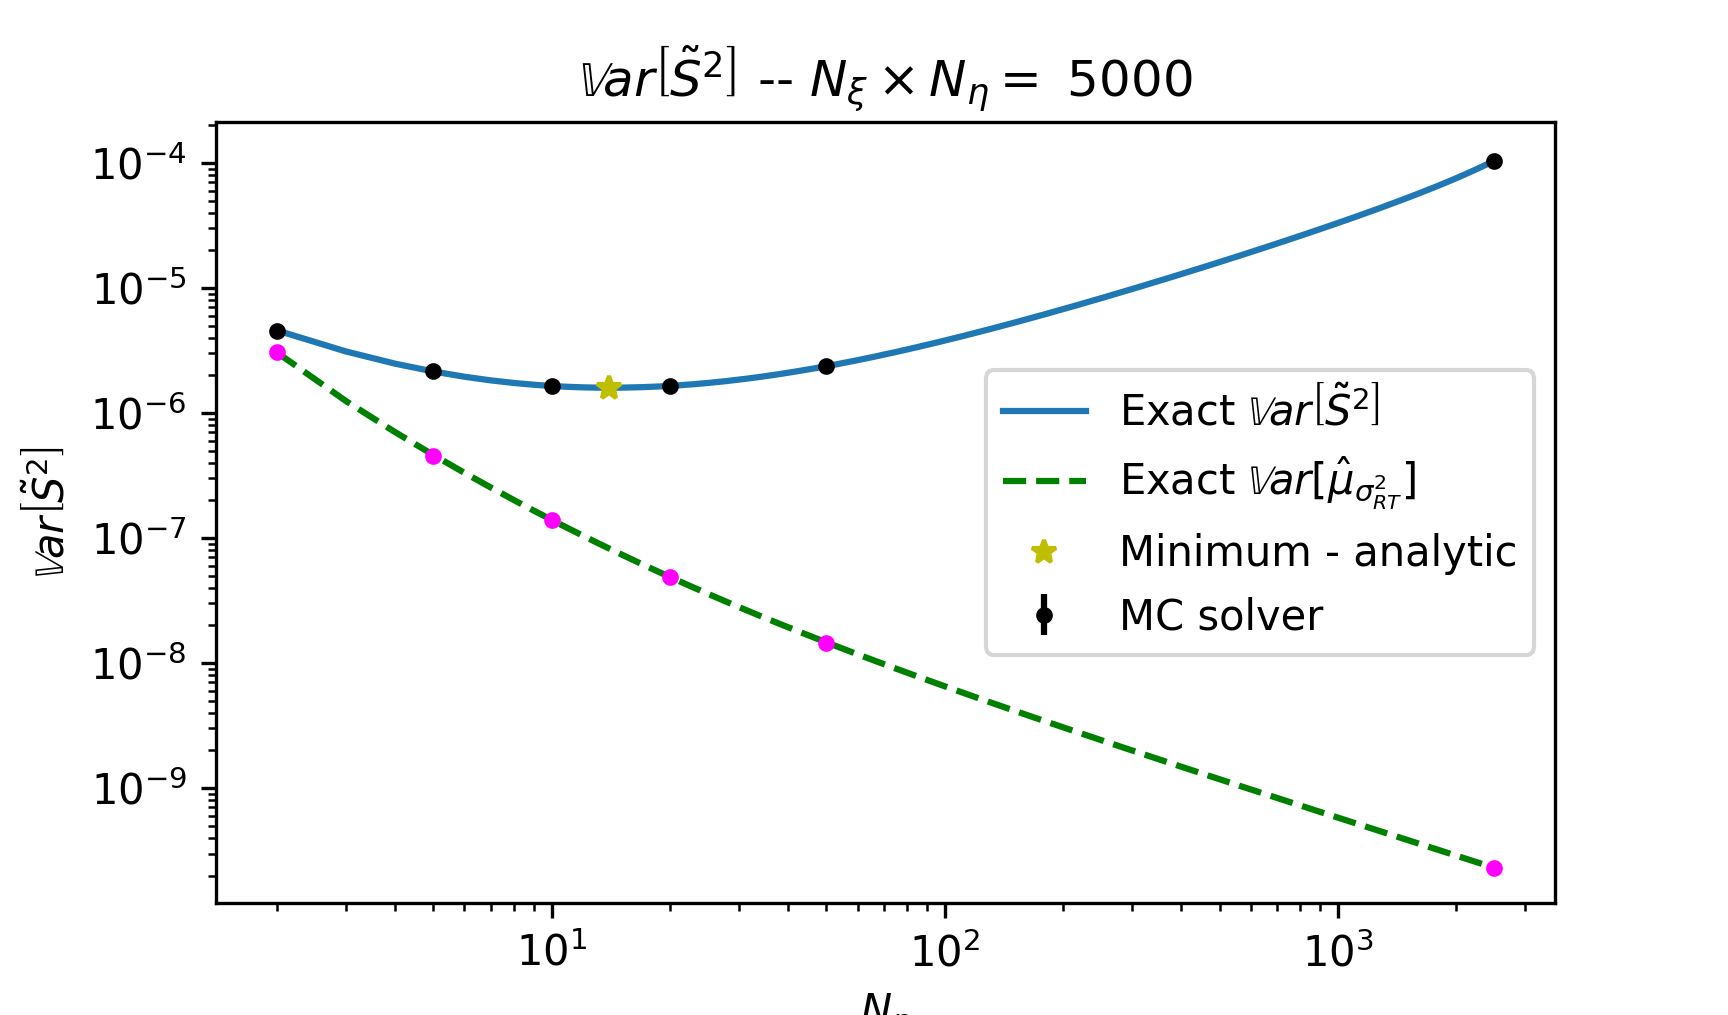
\includegraphics[width=\textwidth]{Figures/log-log.png}
    \caption{$\Var{S^2}$ as a function of $\Neta$ for a variety of total estimator costs, log-log plot. Unfilled point is minimum $\Var{S^2}$. }
    \label{fig:log-log}
\end{figure}

We see a similar trend for the isotropic scattering problem where $S^2$ is $\Var{R}$, the parametric variance of the reflectance tally. However, in this case $\Var{S^2}$ is minimized at $\Neta=20$, rather than $\Neta=10$. While both transmittance and reflectance are influenced by the addition of scattering and the stochastic scattering ratio, the reflectance tally is likely more sensitive to this scattering ratio, and requires more radiation transport tallies to resolve than the transmittance tally. This demonstrates that the optimal number of $\Nxi$ and $\Neta$ can differ between different QoIs even within the same problem, motivating further investigation to allow the analyst to choose these parameters in an informed way. Figure~\ref{fig:compare2000} compares the trends for the attenuation-only estimate of $\Var{T}$ to the isotropic scattering estimate of $\Var{T}$ and $\Var{R}$. 

% $\Var{S^2}$ is minimized for a larger $\Neta$ for reflectance than transmittance for each of the three tested total costs, but a trend is not as discerable as in the attenuation-only case, and further numerical investigation is required for the scattering problem due to its increased stochasticity. 

% The case with isotropic scattering is more complex. Figure \ref{fig:compare2000} shows this same trendline for the total cost $C=2000$, but now comparing the trends for the attenuation-only estimate of $\Var{T}$, the isotropic scattering estimate of $\Var{T}$, and the isotropic scattering estimate of $\Var{R}$. While both estimates of $\Var{T}$ exhibit the same trend for this total cost, we can see that for the isotropic scattering case, $\Var{S^2}$ is minimized when $\Neta=5$, while for the attenuation-only case it's minimized when $\Neta=10$. 
%\textcolor{red}{
% The third line, $\Var{S^2}$ where $S^2$ is an isotropic scattering estimate of $\Var{R}$, does not exhibit a visible trend, particularly for the lower particle histories $\Neta = 2, 5$, and $10$. To understand this, we turn to the physics of the problem. Reflectance as a QoI requires backscattering, and with scattering ratios that can range as low as $c=0.1$, too low of an $\Neta$ makes reflectance difficult to observe. We found $\Var{S^2}$ to be minimized at $\Neta=20$ for the total cost of 2000.
%\textbf{As the scattering case incorporates a larger number of stochastic parameters, the parametric variance becomes a larger contribution to the total polluted variance, and therefore} $\Var{S^2}$ benefits from a higher ratio of $\Nxi$ to $\Neta$ to better resolve the estimate of $S^2$ then in the attenuation-only case.  


\begin{figure}[ht]
    \centering
    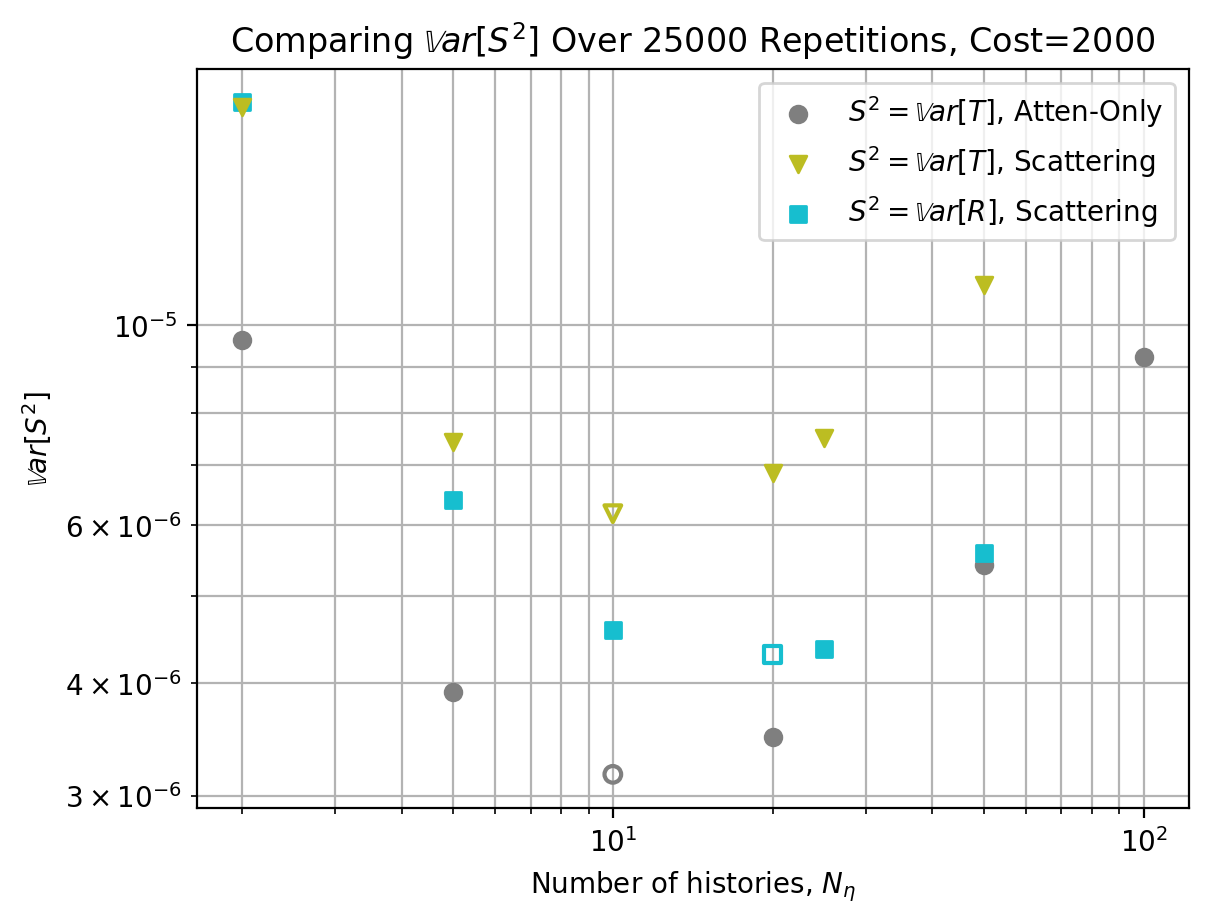
\includegraphics[width=\textwidth]{Figures/2000-scat-vs-atten.png}
    \caption{$\Var{S^2}$ as a function of $\Neta$ for the attenuation-only and scattering cases. Log-log plot, estimator cost $\Nxi \times \Neta=2000$. Unfilled point is minimum $\Var{S^2}$.}
    \label{fig:compare2000}
\end{figure}


\section{Global sensitivity analysis for stochastic solvers}
\subsection{Problem description} \label{sec:closed_form}
To verify the SI method, we can again use an analytic solution for uncollided transmittance of a normally incident beam through a slab from Eq.~\eqref{eq:analytic-trans}. This test problem is a one-dimensional slab with three regions of thicknesses $r_1, r_2$ and $r_3$ and a mono-energetic beam source incident on the first region.
The slab contains three absorption-only materials with total cross sections $\Sigma_{t,1}, \Sigma_{t,2}$ and $\Sigma_{t,3}$.
Region 1 contains $\Nt$ subcells of equal width $\Dx = r_1 / \Nt$, each of which can contain either Material 1 with probability $\PA$ or Material 2 with probability $\left( 1 - \PA \right)$.
The number of cells in Region 1 containing Material 1 in a realization of this stochastic medium can be represented as a sample from the binomial probability density function (PDF), $\NA \sim \mathcal{B}\left( \Nt, \PA \right)$, where $\omega$ represents the non-parametric aleatoric uncertainty of $N_1$.
Region 2 simply contains Material 2.
Region 3 contains Material 3, whose cross section $\Sigma_{t,3}(\xi)$ is a function of parametric aleatoric uncertainty $\xi \sim \mathcal{U}\left(-1, 1 \right)$. 

The problem quantity of interest, transmittance $T$ through the slab, is a function of the optical thickness $\tau$ of each region:
\begin{equation}\label{eq:tau1}
\begin{split}
 \tau_1 &= \NA \Dx \SA + (\Nt - \NA) \Dx \SB \\
    &= \NA \Dx \left( \SA - \SB \right) + r_1 \SB
\end{split}
\end{equation}
\begin{equation}\label{eq:tau2}
    \tau_2 = r_2 \SB
\end{equation}
\begin{equation}\label{eq:tau3}
\begin{split}
 \tau_3 &= r_3\SC = r_3 \left( \StC + \StCd \xi \right) \\
        &= r_3 \StC + r_3 \StCd \xi
\end{split}
\end{equation}
where $\Sigma_{t,3}(\xi)=\Sigma_{t,3}^0+\Sigma_{t,3}^\Delta \xi$, $\StC$ is the mean total cross section, and $\StCd$ the deviation from the mean. The transmittance is therefore a function of both the non-parametric and parametric aleatoric uncertainties, 
\begin{equation}\label{eq:transmission}
 T = \T = k \e{-k_1 N_1(\omega)} \e{-k_3 \xi}
\end{equation}
where
\begin{subequations}\label{eq:constants}
\begin{align}
 &k \hspace{0.13cm}= \exp \left[ -r_1 \SB - r_2 \SB -r_3 \StC \right] \\
 &k_1 = \Dx \left(\SA - \SB \right) \\
 &k_3 = -r_3 \StCd
\end{align}
\end{subequations}

The $p^{th}-$order raw moment of $\T$ is 
%\begin{align}\label{eq:expectation}
%    \EE{\T[p]} &= \EExi{\EEom{\T[p]}} \\
%    &= \int_{\omega} \int_{\xi} d\xi \, d\omega \, 
%    k^p \e{-k_1 p \NA} \e{-k_3 p \xi } \\
%    &= k^p \frac{\sinhh{k_3 p}}{k_3 p} \sum_{x=0}^{\Nt} \Bom \e{-k_1 p x} 
%\end{align}
\begin{equation}\label{eq:expectation}
\begin{split}
    \mathbb{E}_{\xi,\omega}[&T^p(\xi,\omega)] = \EExi{\EEom{\T[p]}} \\
    &= \int_{\omega} \int_{\xi} d\xi \, d\omega \, 
    k^p \e{-k_1 p \NA} \e{-k_3 p \xi } \\
    &= k^p \frac{\sinhh{k_3 p}}{k_3 p} \sum_{x=0}^{\Nt} \Bom \e{-k_1 p x} 
\end{split}
\end{equation}
where $\Bom$ represents the PDF of the binomial variable $\NA$ being equal to $x$:
\begin{equation}
\begin{split}
 \Bom &\defin Pr\left( N_1 = x \g \Nt, \PA \right) \\
 &= \frac{\Nt!}{x! \left( \Nt - x \right)!} \PA^x \left( 1-\PA\right)^{(\Nt-x)}
\end{split}
\end{equation}
%\begin{equation}
% \Bom \defin Pr\left( N_1 = x \g \Nt, \PA \right) = \frac{\Nt!}{x! \left( \Nt - x \right)!} \PA^x \left( 1-\PA\right)^{(\Nt-x)}
%\end{equation}


Eq.~(\ref{eq:expectation}) enables computation of the variance of $\T$ over both aleatoric uncertainties, $\Vxo{\T}$, by expanding the expression for variance,
\begin{equation} \label{eq:closed_var}
    \Vxo{\T} = \EExo{\T[2]} - \EExo{\T[]}^2 .
\end{equation}
This is the denominator of the main and total effect SIs. For comparison with numerical results, we calculate analytic solutions for the numerators in Eqs.~(\ref{eq:SI-xi}) and (\ref{eq:SI-omega}). Taking $\Vxi{\PE(\xi)}$ to indicate the variance of the conditional mean of $\T$ given $\xi$, over all $\xi$, we find that
\begin{equation}
\begin{split} \label{eq:closed_var_cond_mean}
    \Vxi{\PE(\xi)} &= \EExi{\PE^2(\xi)} - \EExi{\PE(\xi)}^2 \\
    &= \EExi{\PE^2(\xi)} - \EExo{\T}^2 .
\end{split}
\end{equation}
The second term is the first-order raw moment of $\T$, calculable from Eq.~(\ref{eq:expectation}). The first term, the second-order raw moment of $\PE(\xi)$, is 

\begin{align}\label{eq:EExi_of_EEomega_sq}
\begin{split}
    \EExi{\PE^2(\xi)} &= \int_{\xi} d\xi \, k^2 \exp(-k_3 \xi) \left( \sum_{x=0}^{\Nt} \Bom \e{-k_1 x} \right)^2 \\
    &= \frac{k^2 \sinhh{2 k_3}}{2 k_3} \left( \sum_{x=0}^{\Nt} \Bom \e{-k_1 x} \right)^2
\end{split}
\end{align}

Inserting Eqs.~(\ref{eq:closed_var}) and (\ref{eq:closed_var_cond_mean}) into Eq.~(\ref{eq:SI-xi}) yields
\begin{equation}
    S_{\xi} = \frac{\frac{k^2 \sinhh{2 k_3}}{2 k_3} \left( \sum_{x=0}^{\Nt} \Bom \e{-k_1 x} \right)^2 - \EExo{\T}^2}{\EExo{\T[2]} - \EExo{\T}^2} \,.
\end{equation}
%\begin{equation}
%    S_{\xi} = \frac{\left( k_3 k^2 \sinhh{2k_3} - 2k^2 \sinh^2\left[k_3\right] \right) \left( \sum_{x=0}^{\Nt} \Bom \exp{-k_1 x}\right)^2}{k_3 k^2 \sinhh{2k_3}\left( \sum_{x=0}^{\Nt} \Bom \e{-2 k_1 x}\right) - 2k^2 \sinh^2\left[k_3\right] \left( \sum_{x=0}^{\Nt} \Bom %\end{equation}
Following the same process to calculate $\Vom{\PE(\omega)}$ yields 
\begin{equation}
    S_{\omega} = \frac{\frac{k^2 \sinh^2 \left[k_3\right]}{k_3^2 } \left( \sum_{x=0}^{\Nt} \Bom \e{-2 k_1 x} \right)  - \EExo{\T}^2}{\EExo{\T[2]} - \EExo{\T}^2} \,.
\end{equation}
Given these closed-form solutions for the main effect SIs, Eqs.~(\ref{eq:SI-xi}) and (\ref{eq:SI-omega}) provide closed-form solutions for the total effect SIs.

%%%%%%%%%%%%%%%%%%%%%%%%%%%%%%%%%%%%%%%%%%%%%%%%%%%%%%%%%%%%%%%%%%%%%%%%%%%%%%%%
\subsection{Numerical results}
We solve two numerical problems each using the problem description from the previous section with $r_1=r_2=r_3=1.0$, $\Sigma_{t,1}=3.0$, $\Sigma_{t,2}=0.1$, $\Sigma_{t,3}^0=1.0$, and $p_1=0.3$. We use two configurations, one with $N_{tot}=10$ and $\Sigma_{t,3}^\Delta=0.25$, and the other with $N_{tot}=100$ and $\Sigma_{t,3}^\Delta=0.75$.
For each quantity on both problems, we use $N_\eta=20$.
For each problem, we first solve for the average transmittance ($\mathbb{E}_{\xi,\omega}\left[T(\xi,\omega)\right]$) and combined aleatoric variance ($\mathbb{V}ar_{\xi,\omega}\left[\Qxo\right]$) using 10,000 samples of the aleatoric uncertainty space (i.e., $\xi$ and $\omega$).
We then use $N_\omega=10$ and $N_\xi=1000$, for a total of 10,000 aleatoric samples, to solve for $\mathbb{V}ar_\xi\left[ \PE(\xi) \right]$.
Next, we use $N_\xi=10$ and $N_\omega=1000$, for a total of 10,000 aleatoric samples, to solve for $\mathbb{V}ar_\omega\left[ \PE(\omega) \right]$.
For each of these numerically computed quantities, we average the computed quantities over 40 repetitions and use those repetitions to compute a standard error of the mean (SEM) for the quantity. To compute SI quantities from the total aleatoric variance and each conditional variance, statistical uncertainties are propagated using the standard error propagation formula for independent variables
\begin{equation}
s_f = \sqrt{  \left( \frac{\partial f}{\partial x} \right)^2 s_x^2 + \left( \frac{\partial f}{\partial y} \right)^2 s_y^2 + \left( \frac{\partial f}{\partial z} \right)^2 s_z^2 + \hdots}.
\end{equation}
\noindent Closed-form values, numerically computed values, and their error compared to the closed-form values are reported in Tables~\ref{tab:pbm1} and~\ref{tab:pbm2} for the first and second problem configurations, respectively. 
\begin{table*}[htb]
    \centering
    \caption{Closed-form and numerically computed results for the $N_{tot}=10$ and $\Sigma_{t,3}^\Delta=0.25$ problem.}
    \begin{tabular}{|l||c|c|r|}\hline
    & \multicolumn{1}{|c|}{Closed} & Numerical & \multicolumn{1}{|c|}{Error}   \\ \hline \hline
    $S_\omega$      & 0.8734261  & 0.8747955 $\pm$ 0.0103919 & $-0.13~\sigma$   \\
    $S_\xi$         & 0.1084529  & 0.1114180 $\pm$ 0.0025490 & $-1.16~\sigma$   \\ \hline
    $S_{T_\omega}$  & 0.8915471  & 0.8885820 $\pm$ 0.0025490 & $1.16~\sigma$    \\
    $S_{T_\xi}$     & 0.1265739  & 0.1252045 $\pm$ 0.0103919 & $0.13~\sigma$    \\
    \hline
    \end{tabular}
\label{tab:pbm1}
\end{table*}

\begin{table*}[htb]
    \centering
    \caption{Closed-form and numerically computed results for the $N_{tot}=100$ and $\Sigma_{t,3}^\Delta=0.75$ problem.}
    \begin{tabular}{|l||c|c|r|}\hline
    & \multicolumn{1}{|c|}{Closed} & Numerical & \multicolumn{1}{|c|}{Error}   \\ \hline \hline\hline \hline
    $S_\omega$          & 0.0873300 & 0.0879516 $\pm$ 0.0026643 & $-0.23~\sigma$  \\
    $S_\xi$             & 0.8968785 & 0.8969538 $\pm$ 0.0083963 & $-0.01~\sigma$ \\ \hline
    $S_{T_\omega}$      & 0.1031215 & 0.1030462 $\pm$ 0.0083963 & $0.01~\sigma$ \\
    $S_{T_\xi}$         & 0.9126700 & 0.9120484 $\pm$ 0.0026643 & $0.23~\sigma$ \\
    \hline
    \end{tabular}
\label{tab:pbm2}
\end{table*}

None of the numerically computed SIs differ from the closed-form solutions by more than 1.16 standard deviations, the error is typically less than 1 standard deviation, and the even distribution between positive and negative error does not suggest a bias. The SIs of these two problems help us understand their practical value: while the transmittance and overall aleatoric variances for each problem are roughly the same, our numerically computed SIs provide a formal mechanism by which to measure that the SM contributes the majority of the variance ($\sim$90\%) in configuration 1 and, by contrast, the uncertain cross section provides the majority of the variance ($\sim$90\%) in configuration 2. Future work with this methodology will include comparing how this algorithm for computing SIs compares with the Saltelli approach outlined in Section~\ref{sec:background-gsa} in accuracy and efficiency.

